%
%  Appendix : Data Analysis Tools
% ================================
%

\chapter{Data Analysis Tools}
\label{Apx:DA}

The simulation codes used in these studies produce large amounts of data.
It has been very useful to develop a tool for effective analysis of both input and output files.
Most of the initial studies were done using OSIRIS 3 (for Publication \ref{Pub:IPAC15} and \ref{Pub:NAPAC16}), and the final emittance study was done using QuickPIC (Publication \ref{Pub:BL17}).

The analysis tools written for these studies are publicly available on GitHub.
The toolbox for OSIRIS 3 is named OsirisAnalysis \cite{code:osiris_analysis:2013}, and the corresponding toolbox for QuickPIC is named QuickPICAnalysis \cite{code:quickpic_analysis:2017}.
Both toolboxes are written for MATLAB.

This appendix briefly outlines the structure and basic function of these tools.

% Also describe briefly how various beam parameters are calculated.
% This should cover Twiss, and the beam quality number used for the last paper.

% ================================================================================================================================ %
\section{The Osiris Analysis Toolbox}
\label{Tools:OA}

The OsirisAnalysis toolbox is a modular and object oriented data analysis toolbox written in MATLAB.
It was designed as a three layer tool to wrap a single data set of OSIRIS simulation data:

\begin{description}
    \item[Layer 1] consists of the core data wrapper class \emph{OsirisData} with its subclass \emph{OsirisConfig}.
        The \emph{OsirisData} class provides an interface for accessing the raw data files, while the \emph{OsirisConfig} class parses the simulation input file.
        \emph{OsirisData} provides a uniform set of calls for extracting the data, and gives through \emph{OsirisConfig} access to all the simulation parameters and conversion factors for converting OSIRIS' normalised units into SI units.
    \item[Layer 2] consists of a set of classes that takes an \emph{OsirisData} object as input, and returns standardised structs\footnote{A \textit{struct} is a type of data structure in programming typically capable of holding a set of values of varying data types. Commonly, as is the case in MATLAB, a struct can contain other structs, allowing data to be stored in a hierarchical manner.} of data that can be scaled and converted to preferred units.
    They perform often needed tools and methods to parse data and extract more detailed information from the larger raw datasets.
    \item[Layer 3] consist of a number of useful standardised plots, and a GUI tool to quickly do a preliminary analysis of simulation data.
\end{description}

The idea behind this layering of the analysis tool is to allow the user to choose how many of these they will use.
Only using the first layer will give the user access to all the simulation parameters as well as a method to extract data in a standardised manner, and return a simple matrix of its content.
Adding the second layer gives additional access to automatic unit conversion and other data conversion tools like slicing and line-outs, as well as various properties extracted from the macro particle arrays.
The third layer provides a quick way to browse through the datasets and display density plots, phase space plots, Twiss parameters, time evolution, etc.

% ================================================================================================================================ %
\subsection{Core Objects}
\label{Tools:OALay1}

The innermost layer consists of two classes:

\begin{description}
    \item[OsirisData:] This class wraps the simulation data folder and is the core interface through which data is extracted.
    The class also provides some simple methods for extracting information about the dataset like physical dimensions of the beam and the distribution of the plasma.
    
    \item[OsirisConfig:] This class is a wrapper for the input file itself, and contains a parser for this file which extracts all the relevant information for both analysis and provides lists of available diagnostics for the graphical user interface (GUI).
    All conversion factors to SI units are calculated on the fly when the input file is loaded.
    The \emph{OsirisConfig} class is not intended to be called by the user, but is found as a child object of the \emph{OsirisData} data object.
\end{description}

% ================================================================================================================================ %
\subsection{Data Types}
\label{Tools:OALay2}

The secondary layer of the OsirisAnalysis framework is a set of subclasses under a parent class named \emph{OsirisType}.
The subclasses will give access to specific types of data more or less directly related to the diagnostics types produced by the OSIRIS simulation code.

The classes provided are:

\begin{description}
    \item[Density and Field:] These are classes that produce grid diagnostics data for the particle density data dumps or the field diagnostics data.
    They support all the different density diagnostics outputs of OSIRIS, and will in addition calculate the wakefields from the magnetic and electric fields given by $W = F/q = E - v \times B$.
    \item[Momentum:] This class consists of a set of methods that will calculate the evolution of the beam's energy and momentum over several time dumps.
    \item[Phase:] This class provides several tools for phase space diagnostics, including calculations of Twiss parameters.
    \item[UDist:] This class is similar to the \emph{Density} and \emph{Field} classes, and provides methods to process velocity and thermal distribution data.
    \item[Species:] This class provides a few additional specialised tools for calculating energy deposition and gain into and from the plasma by the beams, and is also the class where particle tracking data is parsed.
\end{description}

In addition to these data parsing classes, there is also a \emph{Variables} class that will translate OSIRIS diagnostics variables into readable forms, and into strings usable for plot labels.
There is also a \emph{MathFunc} class that provides a math parser that emulates the one used by OSIRIS to parse mathematical functions from the input files.
This class is mainly used to extract geometric information about beam density based on the function provided in the input file without the need to first run the code to provide raw particle data.

% ================================================================================================================================ %
\subsection{Graphical Interface and Plots}
\label{Tools:OALay3}

The final layer of the OsirisAnalysis framework is a set of very flexible plotting tools.
Most of these have a long list of optional input arguments that will change the way data is aggregated and presented.
To make these plots easier to use, most of these optional arguments are available through a graphical interface, also written in MATLAB, named \emph{AnalysisGUI}.

\begin{figure}[hbt]
    \centering
    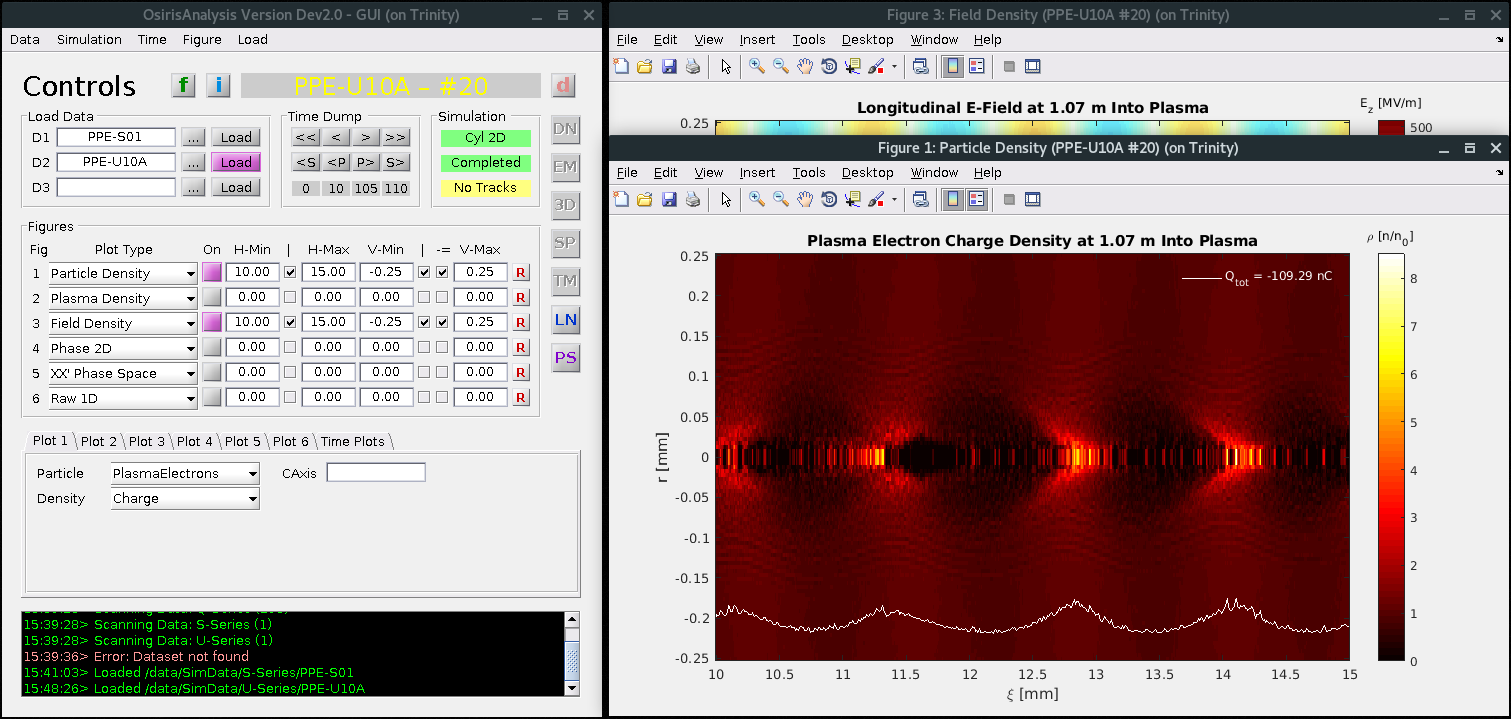
\includegraphics[width=0.99\linewidth,trim={0mm 0mm 0mm 0mm},clip]{images/OsirisAnalysisGUI}
    \caption{\label{Fig:OAGUI} A screen shot of the OsirisAnalysis GUI tool.}
\end{figure}

% ================================================================================================================================ %
\section{QuickPIC Analysis Framework}
\label{Tools:QA}

The toolbox developed for OSIRIS was also partially rewritten to work with QuickPIC simulations.
As QuickPIC uses more or less the same normalised units, the code required little modification to work with these output files.
The conversion was also made easier by QuickPIC having a simpler and more consistent set out output files and formats.

As QuickPIC was only used for the final set of studies, only the core objects and input file wrapper classes, and the data type classes were converted.
No graphical user Interface was developed for this toolbox, and only a few standardised plots were added.
The analysis toolbox is available on GitHub \cite{code:quickpic_analysis:2017}.

% ================================================================================================================================ %
\section{Additional Tools Extending MATLAB Functionality}
\label{Tools:OAAdd}

A number of additional statistics and analysis tools were added due to the lack of MATLAB support, or because alternative methods were beneficial.

\begin{description}
    \item[Weighted Statistics:] Additional functions for weighted mean, percentile and standard deviation used by various parts of both analysis tools were added.
    \item[Weighted Covariance:] The MATLAB \texttt{cov} function does support weighted datasets, but for the OsirisAnalysis tool an exponentially weighted covariance function was used instead \cite{pozzi:2012}.
    This was an attempt to reduce effect of noise in the datasets as this method reduces the impact of statistical outliers.
    For the QuickPIC implementation, the regular MATLAB \texttt{cov} method was used.
    \item[Wavelets:] The Wavelet implementation used in OsirisAnalysis is provided by two script acquired from the websites of The Department of Atmospheric and Oceanic Sciences at The University of Colorado Boulder \cite{torrence:1998}.
\end{description}

